\documentclass{article}
\usepackage[utf8]{inputenc}
\usepackage{graphicx}
\usepackage{appendix}
\usepackage[utf8]{inputenc}
\usepackage[english]{babel}
\usepackage{biblatex}
\usepackage{listings}
\lstset{ 
	language=Matlab,                		% choose the language of the code
%	basicstyle=10pt,       				% the size of the fonts that are used for the code
	numbers=left,                  			% where to put the line-numbers
	numberstyle=\footnotesize,      		% the size of the fonts that are used for the line-numbers
	stepnumber=1,                   			% the step between two line-numbers. If it's 1 each line will be numbered
	numbersep=5pt,                  		% how far the line-numbers are from the code
%	backgroundcolor=\color{white},  	% choose the background color. You must add \usepackage{color}
	showspaces=false,               		% show spaces adding particular underscores
	showstringspaces=false,         		% underline spaces within strings
	showtabs=true,                 			% show tabs within strings adding particular underscores
%	frame=single,	                			% adds a frame around the code
%	tabsize=2,                				% sets default tabsize to 2 spaces
%	captionpos=b,                   			% sets the caption-position to bottom
	breaklines=true,                			% sets automatic line breaking
	breakatwhitespace=false,        		% sets if automatic breaks should only happen at whitespace
	escapeinside={\%*}{*)}          		% if you want to add a comment within your code
}

\addbibresource{ref.bib}
\title{A Simple RBC Model and the Solution Procedure (Adapted)}
\author{Bill Zhu 3150102182}
\date{January 2018}

\begin{document}

\maketitle

\vspace{40pt}
\tableofcontents
\newpage

\section{The Setup}
$$\max E_0\sum_{t=0}^\infty \beta^t \ln(c_t)$$
subject to: 
$$c_t+k_{t+1} = \xi_tk_t^\alpha+(1-\delta)k_t$$
$$\xi_{t+1}=\xi_t^\rho\eta_{t+1}$$
$$\ln\eta_{t+1}\sim(0,\sigma_\eta^2)$$
The Euler conditions are:
$$c_t^{-1}=\beta E_t[c_{t+1}^{-1}(\alpha\xi_{t+1}k_{t+1}^{\alpha-1}+(1-\delta)]$$
$$k_{t+1}=\xi_t k_t^\alpha+(1-\delta)k_t-c_t$$
The transversality condition is:
$$\lim \beta^t\frac{k_t}{c_t} = 0$$
Find the steady state and denote it with no super and subscript.
$$1=\beta [\alpha \xi k^{\alpha-1}+(1-\delta)]$$
$$k=\xi k^\alpha + (1-\delta)k-c$$
Calibration (See Naijing Huang 2012, Table 2.2.1 \& 3.5.1): 
\begin{itemize}
    \item $\alpha=0.36$
    \item $\beta=0.99$
    \item $\rho=0.92$
    \item $\delta=0.02$
    \item $\sigma_\eta=0.006$
\end{itemize}

\newpage
\section{Log-linearize the Euler Equations}
Let $\tilde x_t$ denote $\ln (x_t/x)$. Take log of the Euler equations and linearize around the steady state.
$$ -\tilde c_t = -\tilde c_{t+1}+[1-\beta(1-\delta)][\tilde \xi_{t+1} + (\alpha-1)\tilde k_{t+1}]$$
$$ \tilde k_{t+1}=\frac{1}{\alpha}[\frac{1}{\beta}-(1-\delta)][\tilde \xi_t+\alpha \tilde k_t]+(1-\delta)\tilde k_t+ \{ \delta-\frac{1}{\alpha}[\frac{1}{\beta}-(1-\delta)] \} \tilde c_t$$
$$ \tilde \xi_{t+1}=\rho \tilde \xi_t + \tilde \eta_{t+1}$$
The above equations can be written as:
$$Au_t=BE_t u_{t+1}$$
where
$$u_t= \left[\begin{array}{c} \tilde c_{t} \\ \tilde k_{t} \\ \tilde \xi_{t} \end{array}\right] $$
$$A= \left[\begin{array}{ccc} 1 & 0 & 0 \\ \delta-\frac{1}{\alpha}[\frac{1}{\beta}-(1-\delta)] & 1/\beta & \frac{1}{\alpha}[\frac{1}{\beta}-(1-\delta)] \\
0 & 0 & \rho \end{array}\right]$$
$$B= \left[\begin{array}{ccc} 1 & [1-\beta(1-\delta)](1-\alpha) & -[1-\beta(1-\delta)] \\ 0 & 1 & 0 \\ 0 & 0 & 1 \end{array}\right]$$
solve the matrix we get:
$$A=\left[\begin{array}{ccc} 1 & 0 & 0 \\
-0.063613917 & 1.01010101 & 0.083613917 \\
0 & 0 & 0.92 \end{array}\right]$$
$$B=\left[\begin{array}{ccc} 1 & 0.019072 & -0.0298 \\ 0 & 1 & 0 \\ 0 & 0 & 1 \end{array}\right]$$
Thus,
\begin{equation}
    \left[\begin{array}{c} \tilde c_{t} \\ \tilde k_{t} \\ \tilde \xi_{t} \end{array}\right] = ABE_t
    \left[\begin{array}{c} \tilde c_{t+1} \\ \tilde k_{t+1} \\ \tilde \xi_{t+1} \end{array}\right]
     = CE_t\left[\begin{array}{c} \tilde c_{t+1} \\ \tilde k_{t+1} \\ \tilde \xi_{t+1} \end{array}\right]
\end{equation}
where
$$C=\left[\begin{array}{ccc} 1 & 0.019072 & -0.0298 \\
0.062977778 & 0.991201112 & -0.091852583 \\
0 & 0 & 1.086956522 \end{array}\right]$$
We can transform the above matrix into diagonal form:
$$C=Q \left[\begin{array}{ccc} 1.030535743 & 0 & 0 \\ 0 & 0.960665369 & 0 \\
0 & 0 & 1.086956522 \end{array}\right] Q^{-1}$$
where
$$Q=\left[\begin{array}{ccc} 0.529742466 & -0.436285802 & -0.35396479 \\ 0.848158546 & 0.899808146 & -0.758139979 \\
0 & 0 & 0.547661117 \end{array}\right]$$
and
$$Q^{-1}=\left[\begin{array}{ccc} 1.062716009 & 0.515274182 & 1.400161491 \\
-1.001715387 & 0.625650925 & 0.218673554 \\ 0 & 0 & 1.825946683 \end{array}\right]$$
Thus, multiply the (1) by $Q^{-1}$
$$Q^{-1} \left[\begin{array}{c} \tilde c_{t} \\ \tilde k_{t} \\ \tilde \xi_{t} \end{array}\right] = \left[\begin{array}{ccc} 1.030535743 & 0 & 0 \\ 0 & 0.960665369 & 0 \\ 0 & 0 & 1.086956522 \end{array}\right] Q^{-1}E_t \left[\begin{array}{c} \tilde c_{t+1} \\ \tilde k_{t+1} \\ \tilde \xi_{t+1} \end{array}\right]$$
The eigenvalue which is less than unity implies a linear restriction on $\tilde c_t, \tilde k_t$ and $\tilde \xi_t$. In particular, let,
$$d_t=\left[\begin{array}{ccc} -1.001715387 & 0.625650925 & 0.218673554 \end{array}\right] \left[\begin{array}{c} \tilde c_{t} \\ \tilde k_{t} \\ \tilde \xi_{t} \end{array}\right]$$
Then we have,
\begin{eqnarray*}
    d_t & = & 0.960665369E_t d_{t+1} \\
    & = & 0.960665369E_t d_{t+2} \\
    & = & ... \\
    & = & 0
\end{eqnarray*}
because $d_{t+n} \longrightarrow 0$ as $n \longrightarrow \infty$. In our case, this means,
$$-1.001715387\tilde c_t= 0.625650925\tilde k_t + 0.218673554\tilde \xi_t$$
or
$$\tilde c_t= 0.62457953\tilde k_t + 0.218299086\tilde \xi_t$$
Given this constraint, we can simplify the original 3-dimensional problem to 2-dimensional. \\
Based on (1), now we have
$$\tilde \xi_{t}=1.086956522E_t\tilde \xi_{t+1}$$
\begin{eqnarray*}
    \tilde k_{t+1} & = & -0.063613917(0.62457953\tilde k_t + 0.218299086\tilde \xi_t) + 1.01010101\tilde k_t + 0.083613917\tilde \xi_t \\
    & = & 0.97036906\tilde k_t + 0.069727057\tilde \xi_t
\end{eqnarray*}
Suppose
$$s_t= \left[\begin{array}{c} \tilde k_{t} \\ \tilde \xi_{t} \end{array}\right] $$
Then
\begin{eqnarray*}
s_{t+1} & = & \left[\begin{array}{cc} 0.97036906 & 0.069727057 \\ 0 & 0.92 \end{array}\right] + \left[\begin{array}{c} 0 \\ \tilde \eta_{t} \end{array}\right] \\ & = & Ms_t+\epsilon_{t+1}
\end{eqnarray*}
Suppose
$$z_t= \left[\begin{array}{c} \tilde c_{t} \\ \tilde y_{t} \\ \tilde \iota_{t} \end{array}\right] $$
Note that,
\begin{eqnarray*}
    \tilde y_{t} & = & \alpha \tilde k_{t} + \tilde \xi_{t} \\
    & = & 0.36 \tilde k_t + \xi_t
\end{eqnarray*}
and
\begin{eqnarray*}
    \tilde \iota_{t} & = & (y/i)\tilde y_{t}-(c/i)\tilde c_{t} \\
    & = & 4.180695847\tilde y_{t} -3.180695847\tilde c_{t} \\
    & = & 4.180695847(0.36 \tilde k_t + \xi_t)-3.180695847(0.62457953\tilde k_t + 0.218299086\tilde \xi_t) \\
    & = & -0.481547011 \tilde k_t + 3.48635285 \tilde \xi_t
\end{eqnarray*}
So,
$$\left[\begin{array}{c} \tilde c_{t} \\ \tilde y_{t} \\ \tilde \iota_{t} \end{array}\right]=
\left[\begin{array}{cc} 0.62457953 & 0.218299086 \\ 0.36 & 1 \\ -0.481547011 & 3.48635285 \end{array}\right] s_t
=\Pi s_t$$

\newpage
\section{Computing Impulse Response Functions}
We will use the impulse response functions to describe the responses of endogenous
variables such as $c_{t+j}, y_{t+j} , i_{t+j}$ to technology shock $\epsilon_{t+1}$.
\begin{eqnarray}
    s_{t+j}-E_t s_{t+j} = M^{j-1}\epsilon_{t+1} \\ 
    z_{t+j}-E_t z_{t+j} = \Pi M^{j-1}\epsilon_{t+1}
\end{eqnarray}
It is easy to write a Matlab program to compute the impulse response function (See Appendix).
Here is a figure showing the impulse response functions:
\begin{figure}[ht]
    \centering
    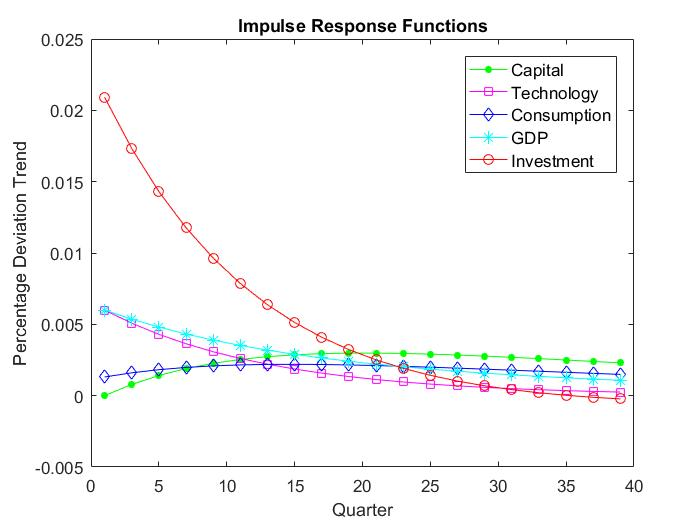
\includegraphics[width=1\textwidth]{1.jpg}
    \caption{Impulse Response Functions}
    \label{fig:1}
\end{figure}

\newpage
\section{Simulation}
We take Huang's estimate in her highly consistent shocks test \cite{Huang}
and set $\sigma_\eta = 0.006$. We use computer-generated normally distributed shocks
and simulate a path for $\tilde\xi$. Assume the economy is initially at the steady state.
The simulated cycle is as follows:
\begin{figure}[ht]
    \centering
    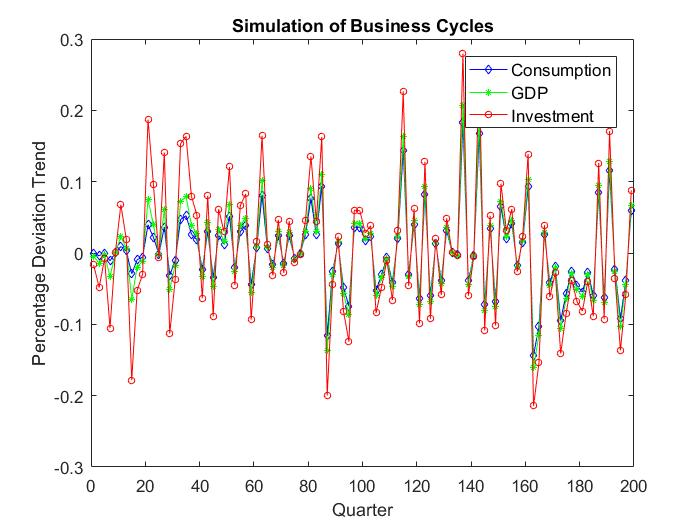
\includegraphics[width=1\textwidth]{2.jpg}
    \caption{Simulation}
    \label{fig:2}
\end{figure}

\newpage
\section{Appendices}
\paragraph{Appendix A: Matlab code}
\noindent
\lstinputlisting[language=Matlab]{fxj1.m}

\newpage
\printbibliography

\end{document}
